\documentclass[review_Solutions]{subfiles}

\IfSubStr{\jobname}{\detokenize{Solutions}}{\toggletrue{solutions}}{\togglefalse{solutions}}

\fancypagestyle{firstpage}

{\rhead{Module 2 Review \linebreak \textit{Version: \today}}}

\title{Module 2: Review of Main Concepts}
\author{Machine Learning}
\date{Fall 2019}

\invalidatemargin

\begin{document}

\maketitle
\thispagestyle{firstpage}

\begin{learningobjectives}
\bi
\item Review some of the key formulas we've learned.
\item Try some practice problems to firm up the details.
\ei
\end{learningobjectives}

\section{Motivation for the Creation of this Document}

Some folks have expressed that they are having a hard time remembering all of the things that they've learned this module.  We are putting this document together to have a single place that lists the main mathematical and algorithms content from this module.  We are aiming for a relatively concise resource, so we are avoiding long explanations.  Eventually, we might (or you might via NB?) add pointers to the original assignments or external resources that explain this stuff more fully.  An exception to this is that in some cases we have put an additional worked example (e.g., in the maximum likelihood estimation section).

\vspace{1em}
\begin{notice}
By creating this document we are not trying to elevate the importance of the math / algorithms portion of this class over the context and ethics or programming parts.  We are creating this resource in response to specific requests from students who wanted more opportunities to reinforce the math and algorithms content.
\end{notice}

\section{What this Document Is and Is Not}

 \paragraph{\textbf{This document is not:}} a standalone resource for learning all of these topics (the explanations provided here are complementary to those given in previous assignments on these same topics), representative of all three streams of the class, a resource for learning new material / concepts not covered in other assignments, something you need to engage with in any particular way (see the next section for some suggestions on how to engage).


 \paragraph{\textbf{This document is:}} a place to assess your understanding of the math and algorithms parts of this module, a place to practice these concepts, a place to ask clarifying / enriching questions (via NB).

\section{How to Engage}

\textbf{You should use this document as a way to solidify concepts which you feel a bit shaky about.}  As a result, if you feel good about a topic, there is no need for you to engage with a particular section.  For instance, if you have the basic idea of probability spaces down, don't even worry about reading that section.  If you would like reinforcement on a topic, read the appropriate section and try some of the practice problems.  You may find it useful to consult the original assignment that introduced these concepts.  Additionally, \textbf{you should post on NB if you have a question or would just like more detail on a particular topic in this document.}


\section{Probability}

\textbf{Probability gives us a formal language to express various forms of uncertainty.}  This is hugely valuable when doing machine learning, which often involves many forms of uncertainty (e.g., missing data, model uncertainty, noise in training data, etc.).

\subsection{Probability Space}
Suppose we want to describe some random process in terms of probability.  To do so, we \textbf{define a probability space}.

A probability space consists of two things.
\bi
\item \textbf{Events:} these are things that may or may not occur as a result a random process.  For example, the event $\mathcal{H}$ might represent the event that when a coin is flipped it comes up heads.
\item \textbf{Probability measure:} this is a function, often called $p$, that assigns a probability to any event.

\noindent In order for $p$ to be a valid probability measure, it must satisfy these three properties.
\be
\item For any event $\mathcal{E}$, $0 \leq p(\mathcal{E}) \leq 1$ (probabilities range from 0, for an impossible event, to 1, for a certain event).
\item For any set of disjoint events, $\mathcal{E}_1, \mathcal{E}_2, \ldots \mathcal{E}_n$ (disjoint events are those that cannot co-occur),
\begin{align}
p(\mathcal{E}_1~\mbox{or}~\mathcal{E}_2 \ldots ~\mbox{or}~\mathcal{E}_n) = \sum_{i=1}^n p(\mathcal{E}_i) \enspace .
\end{align}
\item For any set of exhaustive events, $\mathcal{E}_1, \mathcal{E}_2, \ldots \mathcal{E}_n$ (an exhaustive set of events means at least one \emph{must} occur),
\begin{align}
p(\mathcal{E}_1~\mbox{or}~\mathcal{E}_2 \ldots ~\mbox{or}~\mathcal{E}_n) = 1 \enspace .
\end{align}
\ee
\ei

\begin{exercise}
Consider the random process of rolling a fair, 6-sided die.  Define a probability space (events and a probability measure) to represent this random process.  You can define your own set of events, but an easy default is to define an event for each possible outcome of the roll (e.g., $\mathcal{E}_1$ is the die came out as a 1, $\mathcal{E}_2$ is the die came out as 2, etc.).
\begin{boxedsolution}
Let's define $\mathcal{E}_1, \mathcal{E}_2, \ldots, \mathcal{E}_6$ to be our events.  $\mathcal{E}_i$ represents the event that the die roll comes out with value $i$ (e.g., $\mathcal{E}_3$ means we rolled a 3).  Our probability measure in this case is $p(\mathcal{E}_i) = \frac{1}{6}$ for each of our events.  This function $p$ satisfies the conditions for a probability measure since all events have probability between 0 and 1 and the probability of an exhaustive set of events $p(\mathcal{E}_1~\mbox{or}~\mathcal{E}_2~\ldots~\mbox{or}~\mathcal{E}_6) = \sum_{i=1}^6 p(\mathcal{E}_i) = 1$.
\end{boxedsolution}
\end{exercise}

\begin{exercise}
Construct a probability space to model the 2020 U.S. Congressional Elections.  Define some events of interest (e.g., a particular party controlling one of the houses of congress) and define a valid probability measure over these events (just use your intuition to pick reasonable values, but do adhere to the rules for probability measure specified above).
\begin{boxedsolution}
Let's define the following events and their associated probabilities.
\bi
\item $\mathcal{D_H, R_S}$ is the event that the Democrats control the house and the republicans control the senate (note in this case we've chosen to make this is a single event that entails both of these things happening).  $\mathcal{D_H,D_S}$ is the event that the Democrats control both the house and the senate.  $\mathcal{R_H,R_S}$ is the event that the Republicans control both the house and the senate.  $\mathcal{R_H,D_S}$ is the event that the Republicans control the house and the democrats control the senate.
\item Using the current data on \href{https://www.predictit.org/markets/2/Congress}{predictit} (we didn't expect you to do this, but it is one way to come up with probabilities) $p(\mathcal{D_H, R_S}) = 0.45, p(\mathcal{D_H, D_S}) = 0.29, p(\mathcal{R_H, R_S}) = 0.24, p(\mathcal{R_H, D_S}) = 0.02$.  Notice that these probabilities add to 1 indicating that we are not allowing for any other outcome (since they are disjoint we can add them to get the probability of at least one of them occurring). This gets at the idea that when describing a random process, like an election, using a probability space, we are essentially making modeling decisions about what we consider to be the space of possibilities. For example, In this model we do not allow for a third party to control one of the houses of Congress.
\ei
\end{boxedsolution}
\end{exercise}

\subsection{Random Variables}
A random variable is a generalization of an event.  \textbf{A random variable is an entity that takes on a value as a result of a random process.}  For instance, one might define a random variable $D$ that captures rolling a 6-sided die ($D$ would take on a value from the set $\{1, 2, 3, 4, 5, 6\}$).  (Note: we can also express this random process using events (as we did in the exercise above); both formulations are valid).  A random variable consists of two things.
\bi
\item \textbf{A mapping from each possible outcome of the random process to a value for the random variable} (e.g., our random variable $D$ takes on the value 1 when the die roll comes up 1, value 2 when the die roll comes up 2, etc.).
\item \textbf{A probability mass function (PMF), which gives the probability that a random variable takes on a particular value.}  For example, $p(D = 1)$ is the probability the 6-sided die comes up 1.  If the die is fair, $p(D=1)=\frac{1}{6}$.

\noindent Similar to the conditions outlined for a probability measure, a PMF must satisfy the following conditions.
\be
\item If $V$ is the set of all possible values that the random variable $X$ can take on, then $0 \leq p(X = x) \leq 1$ for any value $x$ in the set $V$.
\item If we add the probability of all possible values that $X$ can take on, we should get $1$.  That is, $\sum_{x \in V} p(X = x) = 1$.
\ee

\ei

\begin{exercise}
Choose a random process and a quantity that would result from that random process.  Define that quantity as a random variable (that is, what values can it take on, what would be a reasonable PMF).  If you pick a pretty simple system you may be able to specify the PMF exactly (e.g., for rolling a die), but for a more complicated problem consider specifying what the PMF looks like at a qualitative level (the solution has an example like this).
\begin{boxedsolution}
Here's one possibility.  Let $W$ be a random variable that represents the number of games that Paul's favorite football team (the San Francisco 49ers) will win over the last 8 games of the regular season.  $W$ can take on any integer in the range $0$ to $8$ (inclusive on both sides).  Since the 49ers are doing well this year (they have won each of their first 8 games), the PMF might peak at $W=6$ (meaning it would be most likely that they will win 6 more games).   Additionally, we know that $p(W=0) + p(W=1) + \ldots + p(W=8) = 1$ since these represent all of the possible values that $W$ can take.
\end{boxedsolution}
\end{exercise}

\begin{notice}
In pretty much all of the content in this module any rule that works for events will also work for random variables.  For instance, Bayes' rule for events $\mathcal{A}$ and $\mathcal{B}$ is $p(\mathcal{A} | \mathcal{B}) = \frac{p(\mathcal{B}|\mathcal{A}) p(\mathcal{A})}{p(\mathcal{B})}$.  This equation looks the same as Bayes' rule for two random variables $X$ and $Y$, $p(X=x | Y=y) = \frac{p(Y=y|X=x) p(X=x)}{p(Y=y)}$.  As a result, when we present a rule for manipulating the probability of various events, you can also assume that it will work with little modification for random variables.  In order to make this document simpler, we won't explicitly give the analogous formula for random variables, but if you have any questions on what it would look like, please post on NB.
\end{notice}

\subsection{Complement Rule}

\noindent If we know the probability of an event $\mathcal{E}$ occurring, then the probability of it not occurring $p(\neg \mathcal{E})$ is given by the formula

\begin{align}
p(\neg \mathcal{E}) = 1 - p(\mathcal{E}) \enspace .
\end{align}

\begin{exercise}
If you flip a fair coin 100 times, the probability of getting all 100 heads is $\left ( \frac{1}{2} \right)^{100}$.  What's the probability of getting at least one tails.
\begin{boxedsolution}
\begin{align}
p(\mbox{at least 1 tails}) &= p(\neg \mbox{100 heads}) \nonumber \\
&= 1 - p(\mbox{100 heads}) \nonumber \\
&= 1 - \left ( \frac{1}{2} \right)^{100}\nonumber
\end{align}
\end{boxedsolution}

\end{exercise}

\subsection{Conditional Probability}
A conditional probability tells us the probability of some event occurring assuming (or conditioned on) another event having occurred.  For instance, we could say ``what is the probability that we observe a particular symptom given that a person has a disease?''  Conditional probability is defined using the following equation.

\begin{align}
p(\mathcal{A}|\mathcal{B}) &= \frac{p(\mathcal{A}, \mathcal{B})}{p(\mathcal{B})}
\end{align}

The term $p(\mathcal{A}, \mathcal{B})$ is known as a joint probability, which we will define in the next section.

\subsection{Joint Probability}
The probability of two events, $\mathcal{A}$ and $\mathcal{B}$, both occurring is called the joint probability of $\mathcal{A}$ and $\mathcal{B}$.  We write this as:
\begin{align}
p(\mathcal{A}, \mathcal{B}) &= \mbox{the probability of both $\mathcal{A}$ and $\mathcal{B}$ simultaneously occurring}
\end{align}

For any two events $\mathcal{A}$ and $\mathcal{B}$, we can write the joint probability in terms of the product of a marginal probability (the probability of one of the events) and a conditional probability.
\begin{align}
p(\mathcal{A}, \mathcal{B}) &= p(\mathcal{A}) p( \mathcal{B} | \mathcal{A})  \\
&= p(\mathcal{B}) p( \mathcal{A} | \mathcal{B})
\end{align}


\subsection{Marginalization}
If we can easily compute the joint distribution of two events (that is $p(\mathcal{A}, \mathcal{B})$), then we can use the technique of marginalization to obtain the \emph{marginal distribution} (the probability of just one of the events in isolation).

\begin{align}
p(\mathcal{A}) &= p(\mathcal{A}, \mathcal{B}) + p(\mathcal{A}, \neg \mathcal{B})
\end{align}


Another way to think about marginalization is to draw a tree.  For example, this is tree from a previous assignment that described the process of choosing between two coins ($\mathcal{C}_1$ and $\mathcal{C}_2$) and flipping the chosen coin twice.  The first coin is fair and the second coin is biased (probability of heads is 4/5).

\begin{center}
\includegraphics[width=0.8\linewidth]{../02/figures/twocoins}
\end{center}

If we want to compute the marginal probability of any of the events $\mathcal{H}_1, \mathcal{H}_2, \mathcal{C}_1, \mathcal{C}_2$, we can simply add the probability of each path that contains the event of interest.  The probability of a path is the product of the probabilities along it.

For example,
\begin{align}
p(\mathcal{H}_2) &= p(\mathcal{C}_1, \mathcal{H}_1, \mathcal{H}_2) + p(\mathcal{C}_1, \neg \mathcal{H}_1, \mathcal{H}_2) + p(\mathcal{C}_2, \mathcal{H}_1, \mathcal{H}_2) + p(\mathcal{C}_2, \neg \mathcal{H}_1, \mathcal{H}_2) \nonumber \\
&= \left ( \frac{1}{2} \times \frac{1}{2} \times \frac{1}{2} \right) + \left ( \frac{1}{2} \times \frac{1}{2} \times \frac{1}{2} \right) + \left ( \frac{1}{2} \times \frac{4}{5} \times \frac{4}{5} \right) + \left ( \frac{1}{2} \times \frac{1}{5} \times \frac{4}{5} \right) \nonumber \\
&= \frac{1}{8} + \frac{1}{8} + \frac{8}{25} + \frac{2}{25} \nonumber \\
&= \frac{13}{20} \nonumber
\end{align}


It's worth giving the translation of this to random variables explicitly.  If $X$ and $Y$ are random variables and $V$ contains all possible values that $X$ can take on, then
\begin{align}
p(Y=y) &= \sum_{x \in V} p(Y=y, X=x) \enspace .
\end{align}

\begin{exercise}
Let's define the event $\mathcal{D}$ as the two flips in the coin problem above having different outcomes (e.g., one is heads and one is tails).  Using the technique of marginalization, what is $p(\mathcal{D})$?  If it helps, consider augmenting the tree of the coin problem to list either $\mathcal{D}$ or $\neg \mathcal{D}$ at the end of each path.  Here is what it might look like.

\begin{center}
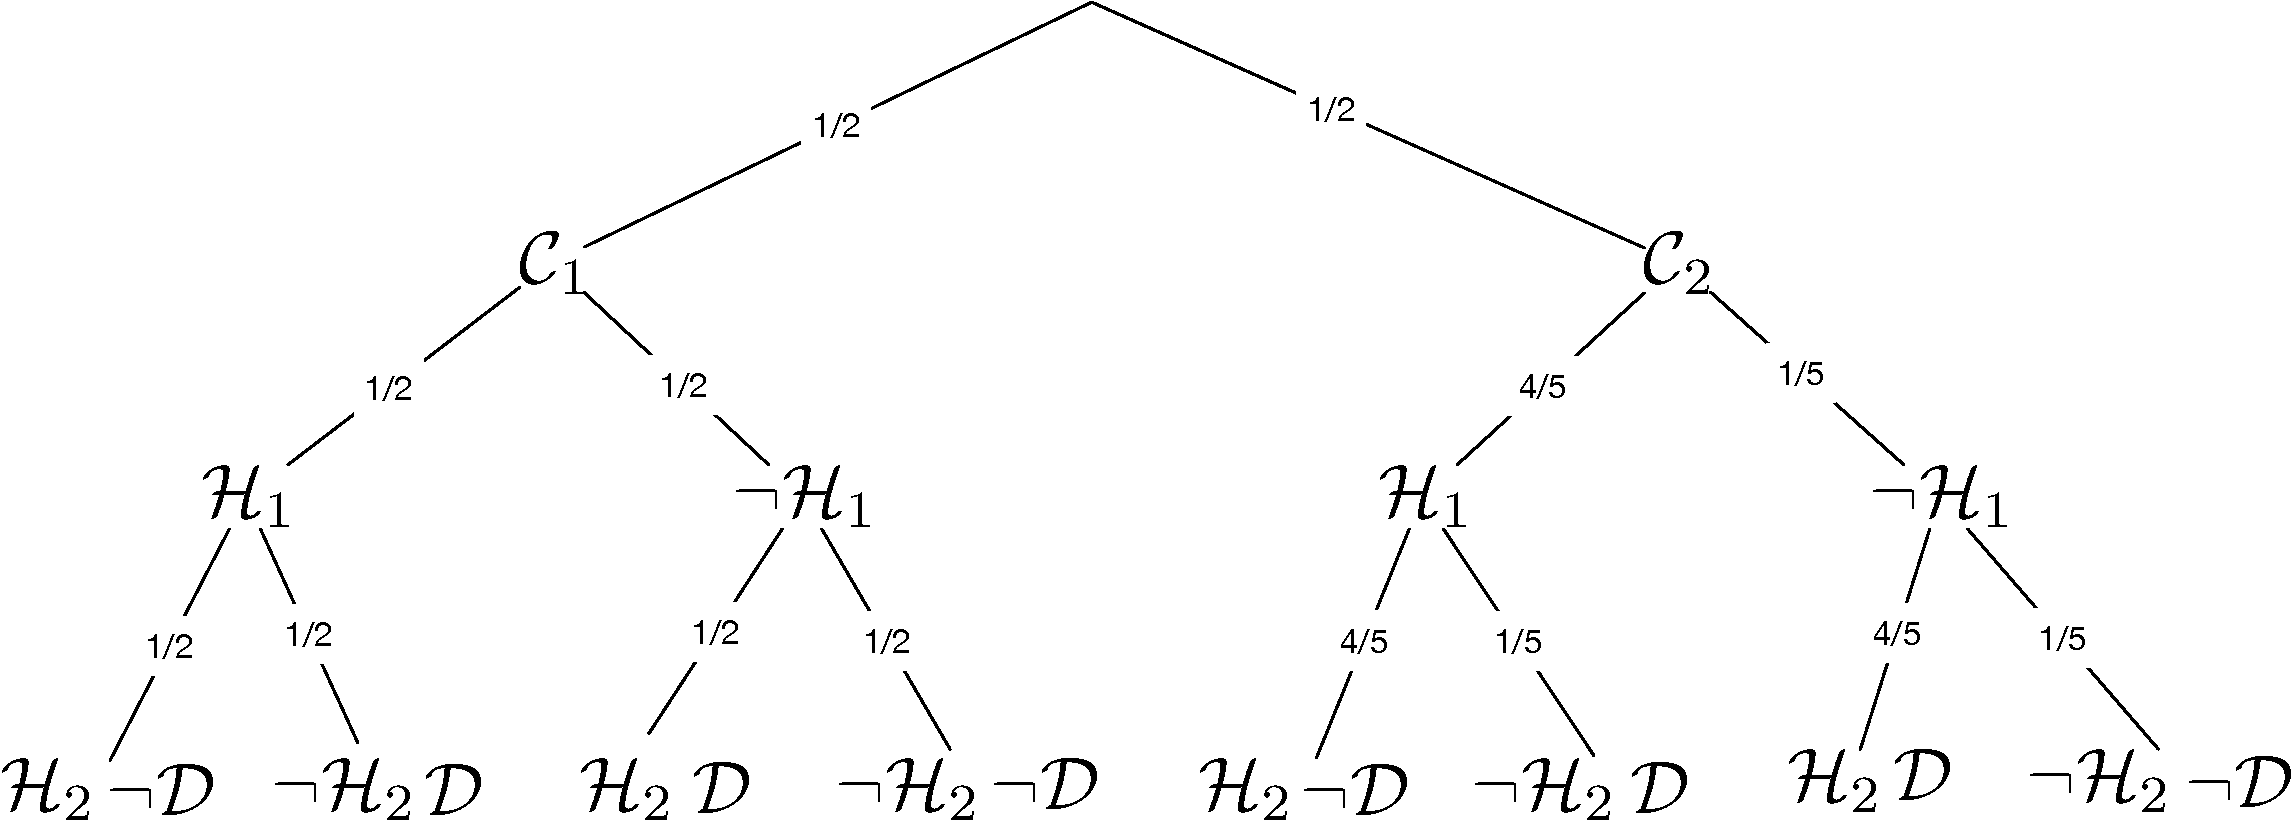
\includegraphics[width=0.8\linewidth]{figures/twocoins_with_diff}
\end{center}
\begin{boxedsolution}
We can find the probability by summing the probability of all of the paths that lead to $\mathcal{D}$.
\begin{align}
p(\mathcal{D}) &= p(\mathcal{C}_1, \mathcal{H}_1, \neg \mathcal{H}_2) + p(\mathcal{C}_1,\neg \mathcal{H}_1, \mathcal{H}_2) + p(\mathcal{C}_2, \mathcal{H}_1, \neg \mathcal{H}_2) + p(\mathcal{C}_2,\neg \mathcal{H}_1, \mathcal{H}_2) \nonumber \\
&= \left ( \frac{1}{2} \times \frac{1}{2} \times \frac{1}{2} \right) +  \left ( \frac{1}{2} \times \frac{1}{2} \times \frac{1}{2} \right) +  \left ( \frac{1}{2} \times \frac{4}{5} \times \frac{1}{5} \right) +  \left ( \frac{1}{2} \times \frac{1}{5} \times \frac{4}{5} \right) \nonumber \\
&= \frac{41}{100} \nonumber
\end{align}
\end{boxedsolution}
\end{exercise}


\subsection{Product Rule}

We can decompose the joint probability of a bunch of events into a product of probabilities.  Suppose $\mathcal{E}_1, \mathcal{E}_2, \ldots, \mathcal{E}_n$ represent events, then
\begin{align}
p(\mathcal{E}_1, \mathcal{E}_2, \ldots, \mathcal{E}_n) &= p(\mathcal{E}_1) p(\mathcal{E}_2 | \mathcal{E}_1) p(\mathcal{E}_3 | \mathcal{E}_1, \mathcal{E}_2) \ldots p(\mathcal{E}_n | \mathcal{E}_1, \ldots, \mathcal{E}_{n-1}) \enspace .
\end{align}
The rule we're applying here is to start with an event conditioned on nothing, then multiply by the next event conditioned on the previous event, then multiply by the next event conditioned on the previous two, etc.  The order in which you select the events is also arbitrary, so if $n=3$, the following are equivalent.
\begin{align}
p(\mathcal{E}_1, \mathcal{E}_2, \mathcal{E}_3) &= p(\mathcal{E}_1) p(\mathcal{E}_2|\mathcal{E}_1)p(\mathcal{E}_3|\mathcal{E}_1, \mathcal{E}_2) \nonumber \\
&= p(\mathcal{E}_2) p(\mathcal{E}_3|\mathcal{E}_2)p(\mathcal{E}_1|\mathcal{E}_2, \mathcal{E}_3) \nonumber \\
&= p(\mathcal{E}_3) p(\mathcal{E}_2|\mathcal{E}_3)p(\mathcal{E}_1|\mathcal{E}_3, \mathcal{E}_2) \nonumber \\
&\mbox{... there are three more potential orderings that we won't give explicitly} \nonumber
\end{align}

\begin{exercise}
Here is a \href{https://www.khanacademy.org/math/ap-statistics/probability-ap/probability-multiplication-rule/e/dependent\_probability}{review problem from Khan academy} that can be solved most straightforwardly using the product rule.

\begin{quote}
A goblet contains 3 red balls, 2 green balls, and 6 blue balls.

If we choose a ball, then another ball without putting the first one back in the goblet, what is the probability that the first ball will be red and the second will be blue?
\end{quote}
\begin{boxedsolution}
Let's define the event the first ball is red as $\mathcal{R}_1$ and the event that the second ball is blue as $\mathcal{B}_2$.
\begin{align}
p(\mathcal{R}_1, \mathcal{B}_2) &= p(\mathcal{R}_1) p(\mathcal{B}_2 \mid \mathcal{R}_1) \nonumber \\
&= \frac{3}{11} \times \frac{6}{10} \nonumber \\
&= \frac{9}{55} \nonumber
\end{align}
\end{boxedsolution}
\end{exercise}

\subsection{Bayes' Rule}

Bayes' rule lets you take a conditional probability $p(\mathcal{A}|\mathcal{B})$ and flip the order of the events across the conditioning bar.
\begin{align}
p(\mathcal{A}|\mathcal{B}) &= \frac{p(\mathcal{B}|\mathcal{A}) p(\mathcal{A})}{p(\mathcal{B})}
\end{align}

There are a few alternate forms of Bayes' rule.
\bi
\item You can move multiple events through the conditioning bar (here are two examples where we move two events, but you can move any number of events).
\begin{align}
p(\mathcal{A}, \mathcal{B} | \mathcal{C}) &= \frac{p(\mathcal{C}|\mathcal{A}, \mathcal{B}) p(\mathcal{A}, \mathcal{B})}{p(\mathcal{C})} \\
p(\mathcal{A} |  \mathcal{B}, \mathcal{C}) &= \frac{p(\mathcal{B}, \mathcal{C}|\mathcal{A}) p(\mathcal{A})}{p(\mathcal{B}, \mathcal{C})}
\end{align}
\item You don't have to swap all of the events across the conditioning bar (e.g., below, we leave $\mathcal{C}$ on the righthand side of the bar).
\begin{align}
p(\mathcal{A}|\mathcal{B},\mathcal{C}) &= \frac{p(\mathcal{B} | \mathcal{A}, \mathcal{C}) p(\mathcal{A}|\mathcal{C})}{p(\mathcal{B}|\mathcal{C})}
\end{align}
\ei


\paragraph{What's the big deal about Bayes?}
Here are two potential answers to this.
\bi
\item \textbf{It helps us compute probabilities of interest.}  Sometimes it is much more natural to compute $p(\mathcal{B} | \mathcal{A})$, then $p(\mathcal{A} | \mathcal{B})$.  For example, if $\mathcal{A}$ represents the event that someone has a particular disease and $\mathcal{B}$ represents someone exhibiting a particular symptom, since we think of the disease as causing the symptom it may be easier to model the probability of the symptom given the disease.  It is less natural to think of the probability of the disease given the symptom since we don't typically think of a symptom as causing a disease.
\item Consider watching Julia Galef's \href{https://www.youtube.com/watch?v=za7RqnT7CM0}{Bayes: How one equation changed the way I think}.
\ei

\begin{exercise}
There are lots of practice problems on the web for Bayes' rule.  Here are some suggestions.
\bes
\item Former Olin Professor Sanjoy Mahajan has a bunch of practice problems on Bayes' rule available on his website.  Each problem allows you to submit your answer and have it checked automatically.  He also has the solution for each problem posted.  Some of the problems are more standalone than others (e.g., some rely on material communicated in class).  We'll suggest some that seem to be standalone here.  First, visit the \href{https://tutor.sanjoymahajan.org/bayes/hw02}{HW02 page on Sanjoy's website} (if you get a privacy error from your browser, go ahead and allow your browser to access the site.  What could go wrong?).  On this page, consider doing \textbf{problem 2} (this one is using Bayes' rule in reverse, so it is a bit of a twist), \textbf{problem 3} (part (a) is really a question about marginalization), \textbf{problem 4}, and \textbf{problem 5}.
\begin{boxedsolution}
The solutions are already on Sanjoy's website.
\end{boxedsolution}
\item Here are \href{http://www2.stat.duke.edu/~jerry/sta101/extraproblems/bayesian.htm}{some more practice problems} from a class on Bayesian statistics.
\begin{boxedsolution}
Solutions available upon request.
\end{boxedsolution}
\ees
\end{exercise}


\subsection{Independence}

Two events $\mathcal{A}$ and $\mathcal{B}$ are independent (written as $\mathcal{A} \condindep \mathcal{B}$) if and only if
\begin{align}
p(\mathcal{A}, \mathcal{B}) = p(\mathcal{A}) p(\mathcal{B}) \enspace .
\end{align}
This equation also implies the following very useful rule.
\begin{align}
p(\mathcal{A} | \mathcal{B}) = p(\mathcal{A}) \enspace .
\end{align}
Intuitively, we can drop $\mathcal{B}$ from the right side of the conditioning bar since knowing that $\mathcal{B}$ occurred doesn't change the probability of $\mathcal{A}$.

\begin{exercise}
Simplify each expression using the fact that $\mathcal{A} \condindep \mathcal{B}$ and $\mathcal{C} \condindep \mathcal{D}$ (don't worry about doing anything fancy, just apply the product rule and the basic definitions of independence above).  To make things simpler, assume that these independence relationships hold no matter what events you condition on.
\bes
\item $p(\mathcal{A} | \mathcal{B}, \mathcal{C})$
\begin{boxedsolution}
This one is an application of the fact that you can drop an event from the right side of the conditioning bar if it is conditionally independent of the events on the left side of the conditioning bar.
\begin{align}
p(\mathcal{A} | \mathcal{B}, \mathcal{C}) &= p(\mathcal{A} | \mathcal{C})
\end{align}
\end{boxedsolution}
\item $p(\mathcal{A}, \mathcal{B}, \mathcal{C})$
\begin{boxedsolution}
Use the product rule to expand.  Depending on the order you chooses to expand, you will get a slightly different, but equivalent, answer.
\begin{align}
p(\mathcal{A}, \mathcal{B}, \mathcal{C}) &= p(\mathcal{A}) p(\mathcal{B}| \mathcal{A}) p(\mathcal{C} | \mathcal{A}, \mathcal{B}) \nonumber \\
&= p(\mathcal{A}) p(\mathcal{B}) p(\mathcal{C} | \mathcal{A}, \mathcal{B}) \nonumber
\end{align}
\end{boxedsolution}
\ees
\end{exercise}

\subsection{Conditional Independence}


Two events $\mathcal{A}$ and $\mathcal{B}$ are conditionally independent given a third event $\mathcal{C}$ (written as $\mathcal{A} \condindep \mathcal{B}~|~\mathcal{C}$) if and only if
\begin{align}
p(\mathcal{A}, \mathcal{B} | \mathcal{C}) = p(\mathcal{A} | \mathcal{C}) p(\mathcal{B} | \mathcal{C}) \enspace .
\end{align}
This equation also implies the following very useful rule.
\begin{align}
p(\mathcal{A} | \mathcal{B}, \mathcal{C}) = p(\mathcal{A} | \mathcal{C}) \enspace .
\end{align}
The intuition is that we can drop $\mathcal{B}$ from the right side of the conditioning bar since knowing that $\mathcal{B}$ occurred doesn't change the probability of $\mathcal{A}$ if we already know that $\mathcal{C}$ occurred.


\begin{exercise}
Suppose we know the following facts about some events $\mathcal{A}, \mathcal{B}, \mathcal{C}, \mathcal{D}$.
\bi
\item $\mathcal{A} \condindep \mathcal{B}$
\item $\mathcal{A} \condindep \mathcal{C} \mid \mathcal{B}$
\item $\mathcal{A} \condindep \mathcal{D} \mid \mathcal{C}$
\ei

\noindent Simplify the expression $p(\mathcal{A}, \mathcal{B}, \mathcal{C}, \mathcal{D})$ as much as possible (again, don't worry about doing anything fancy, just apply the product rule and the basic definitions of independence and conditional independence above).

\begin{boxedsolution}
\begin{align}
p(\mathcal{A}, \mathcal{B}, \mathcal{C}, \mathcal{D}) &= p(\mathcal{A}) p(\mathcal{B}|\mathcal{A}) p(\mathcal{C} | \mathcal{A}, \mathcal{B}) p(\mathcal{D}|\mathcal{A}, \mathcal{B}, \mathcal{C}) & \mbox{product rule} \nonumber \\
&= p(\mathcal{A}) p(\mathcal{B})p(\mathcal{C} | \mathcal{A}, \mathcal{B}) p(\mathcal{D}|\mathcal{A}, \mathcal{B}, \mathcal{C}) & A \condindep B \nonumber \\
&= p(\mathcal{A}) p(\mathcal{B})p(\mathcal{C} |\mathcal{B}) p(\mathcal{D}|\mathcal{A}, \mathcal{B}, \mathcal{C}) & \mathcal{A} \condindep \mathcal{C} \mid \mathcal{B} \nonumber \\
&=  p(\mathcal{A}) p(\mathcal{B})p(\mathcal{C} |\mathcal{B}) p(\mathcal{D}| \mathcal{B}, \mathcal{C}) & \mathcal{A} \condindep \mathcal{D} \mid \mathcal{C}\nonumber
\end{align}
\end{boxedsolution}
\end{exercise}

\section{Bayesian Networks}

A Bayesian Network (BN) defines a model consisting of one or more events or random variables.  A BN consists of the following components.
\bi
\item A \textbf{graph, that encodes the dependencies between one or more random variables and events.}  This graph contains nodes that represent random variables or events and directed edges that indicate causal relationships between nodes (e.g., an edge from from node $A$ to node $B$ indicates that $A$ causes $B$).
\item A \textbf{conditional probability table that indicates the probability that a node takes on a particular value given the values of its parents.}
\ei

Here is an example of a BN that represents how two people, Mary and John, respond to an alarm in their apartment complex.  The alarm is triggered by earthquakes and burglaries.

\begin{center}
\includegraphics[width=0.6\linewidth]{../02/figures/maryjohn}
\end{center}

The circles in this graph (called nodes) are the various events.  Each of these can either be true or false (as stated before, nodes can also represent random variables that can take on multiple values).  The arrows indicate causal relationships (e.g., the alarm going off is caused by burglaries and earthquakes).  The tables next to each node give us the probability of the node conditioned on its parents.

 The condition that must hold for any BN is that if we write the joint distribution of all of the random variables (or events, since the relationship is the same for either) in the network, it must factorize in the following way (we'll use $X_1, X_2, \ldots X_n$ to represent random variables in the network and we'll define the function $Pa(X_i)$ to return all of the random variables that are parents of $X_i$).

\begin{align}
p(X_1, X_2, \ldots, X_n) &= p(X_1 | Pa(X_1)) p(X_2 | Pa(X_2)) \ldots p(X_n | Pa(X_n)) \label{eq:bnparents}
\end{align}

\begin{exercise}
For practice, use Equation~\ref{eq:bnparents} to factor $p(\mathcal{B}, \mathcal{E}, \mathcal{A}, \mathcal{J}, \mathcal{M})$ for the alarm network.
\begin{boxedsolution}
\begin{align}
p(\mathcal{B}, \mathcal{E}, \mathcal{A}, \mathcal{J}, \mathcal{M}) &= p(\mathcal{B}) p(\mathcal{E}) p(\mathcal{A} | \mathcal{B}, \mathcal{E}) p(\mathcal{J} | \mathcal{A}) p(\mathcal{M} | \mathcal{A})   \nonumber
\end{align}
\end{boxedsolution}
\end{exercise}



\subsection{D-Separation}
One of the beautiful things about BNs is that they allow us to infer independence relationships from the graph structure.  In assignment 2 we gave some resources to learn about d-separation.  We encourage you to take a second look at those if you are having trouble (one was a video and one was a document).  If you find any other good resources on d-separation, please share them here.  Next, we'll try to state the rules of d-separation as clearly and concisely as possible.
\vspace{1em}
\begin{recall}[Definition of D-Separation]
Two nodes, $\mathcal{A}$ and $\mathcal{B}$, in a BN are d-separated when conditioning on a set of nodes, $\mathcal{C}$, if and only if \emph{all} paths between  $\mathcal{A}$ and $\mathcal{B}$ are blocked when conditioning on $\mathcal{C}$ (the concept of \emph{blocked} will be defined below).  Note that a path consists of traversing one or more edges, in sequence, of a BN (irrespective of the direction of the edge).  A path between $\mathcal{A}$ and $\mathcal{B}$ conditioned on nodes $\mathcal{C}$ \textbf{is blocked if any of the following conditions are met}.
\be
\item The path contains a collider and neither the collider nor any of its descendants are in the set $\mathcal{C}$ (a collider is a node where the path consists of two incoming arrows, e.g., $\mathcal{D} \rightarrow \mathcal{E} \leftarrow \mathcal{F}$).
\item The path contains a segment that looks like $\mathcal{D} \rightarrow \mathcal{E} \rightarrow \mathcal{F}$ and $\mathcal{E}$ is in the set $\mathcal{C}$ (i.e., we are conditioning on $\mathcal{E}$).
\item The path contains a segment that looks like $\mathcal{D} \leftarrow \mathcal{E} \rightarrow \mathcal{F}$ and $\mathcal{E}$ is in the set $\mathcal{C}$ (i.e., we are conditioning on $\mathcal{E}$).
\ee


\vspace{1em}
\noindent If $\mathcal{A}$ and $\mathcal{B}$ are d-separated conditioned on $\mathcal{C}$, then $\mathcal{A} \condindep \mathcal{B}~|~\mathcal{C}$.

\end{recall}

\begin{exercise}
Choose two nodes in the alarm network.  Are they independent?  How would this change if you conditioned on each of the other three nodes in the network?  Repeat this exercise for other pairs of nodes in the network.
\begin{boxedsolution}
As an example, let's pick $\mathcal{E}$ and $\mathcal{B}$.  We can use d-separation to determine the independence and conditional independence relationships.
\bi
\item $\mathcal{E} \condindep \mathcal{B}$ ($\mathcal{A}$ is a collider and blocks the only path between $\mathcal{E}$ and $\mathcal{B}$).
\item $\mathcal{E} \notcondindep \mathcal{B}~|~\mathcal{A}$ (the slash through $\condindep$ means that the two nodes are not conditionally independent given $\mathcal{A}$).  Since we are conditioning on $\mathcal{A}$, the fact that it is a collider no longer blocks the path between $\mathcal{E}$ and $\mathcal{B}$.
\item $\mathcal{E} \notcondindep \mathcal{B}~|~\mathcal{J}$.  Since we are conditioning on $\mathcal{J}$, which is a descendant of $\mathcal{A}$, even though $\mathcal{A}$ is a collider it no longer blocks the path between $\mathcal{E}$ and $\mathcal{B}$.
\item $\mathcal{E} \notcondindep \mathcal{B}~|~\mathcal{M}$.  Since we are conditioning on $\mathcal{M}$, which is a descendant of $\mathcal{A}$, even though $\mathcal{A}$ is a collider it no longer blocks the path between $\mathcal{E}$ and $\mathcal{B}$.
\ei
\end{boxedsolution}
\end{exercise}


\begin{exercise}
Consider this network that describes the operation of various parts of a car (this is from \href{http://idm-lab.org/intro-to-ai/slides/Bayesian\_Networks.pdf}{Slide 20 of Sven Koenig's lecture on Bayesian Networks}).

\begin{center}
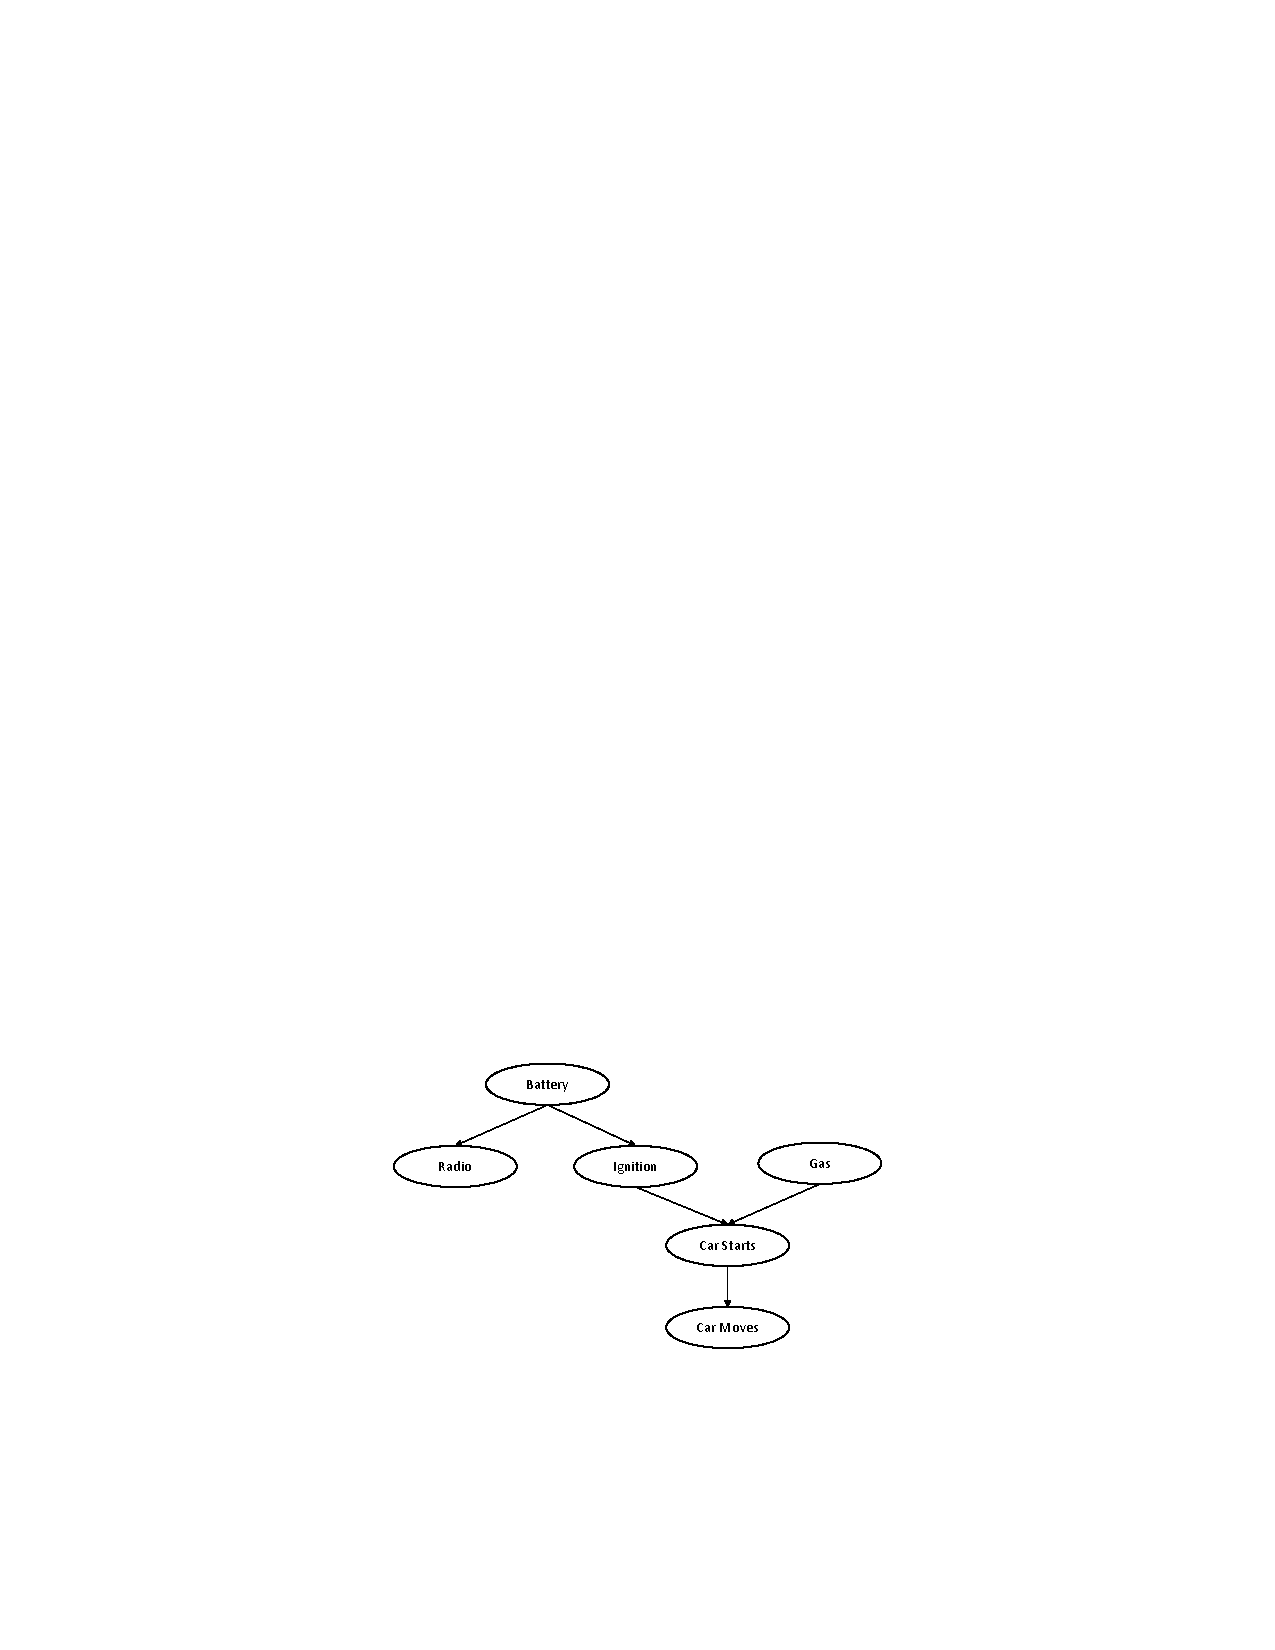
\includegraphics[width=0.6\linewidth]{figures/carnetwork}
\end{center}

Using the rules of d-separation, determine whether the following conditional independence relationships are true or false (excuse the upper case letters, the cool calligraphic math font doesn't support lowercase letters).
\bi
\item $\mathcal{RADIO} \condindep \mathcal{IGNITION}$?
\begin{boxedsolution}
False.  The path between them doesn't contain a collider or a node that we are conditioning on that would block the path. 
\end{boxedsolution}
\item $\mathcal{RADIO} \condindep \mathcal{IGNITION}\mid\mathcal{BATTERY}$?
\begin{boxedsolution}
True.  The path between is blocked by conditioning on $\mathcal{BATTERY}$.
\end{boxedsolution}
\item $\mathcal{RADIO} \condindep \mathcal{GAS}$?
\begin{boxedsolution}
True.  The path between is blocked by the collider $\mathcal{CAR STARTS}$.
\end{boxedsolution}
\item $\mathcal{RADIO} \condindep \mathcal{GAS}\mid\mathcal{CAR MOVES}$?
\begin{boxedsolution}
False.  The path is no longer blocked by the collider $\mathcal{CAR STARTS}$ because we are conditioning on $\mathcal{CAR MOVES}$, which is a descendent of $\mathcal{CAR STARTS}$.
\end{boxedsolution}
\item This one is a pretty rich network.  You could keep going to create new practice problems.
\ei
\end{exercise}

\begin{exercise}
Consider the following BN that represents a situation facing a doctor trying to diagnose a newborn that comes into the hospital with a fever.  In this scenario there are two possible underlying diagnoses that could cause this symptom of having a fever (represented by the event $\mathcal{F}$): a common cold virus (represented by the event $\mathcal{C}$) or meningitis (represented by the event $\mathcal{M}$).

% another idea from Kaitlyn
% (Rank most to least prevalent for a 7 year old): 1, 2, 4, 3
% Common cold (URI) (1), Pneumonia (2), Bronchitis (3), Asthma (4)
% Cough (1, 2, 3, less of 4), Chest pain (rank high to low: 2, 4, 3, 1), Wheezing (high to low 4, 3, 2, 1), shortness of breath (high to low 4, 2, 3, 1)
Note: these are not real numbers, but display some of the correct trends.

\begin{center}
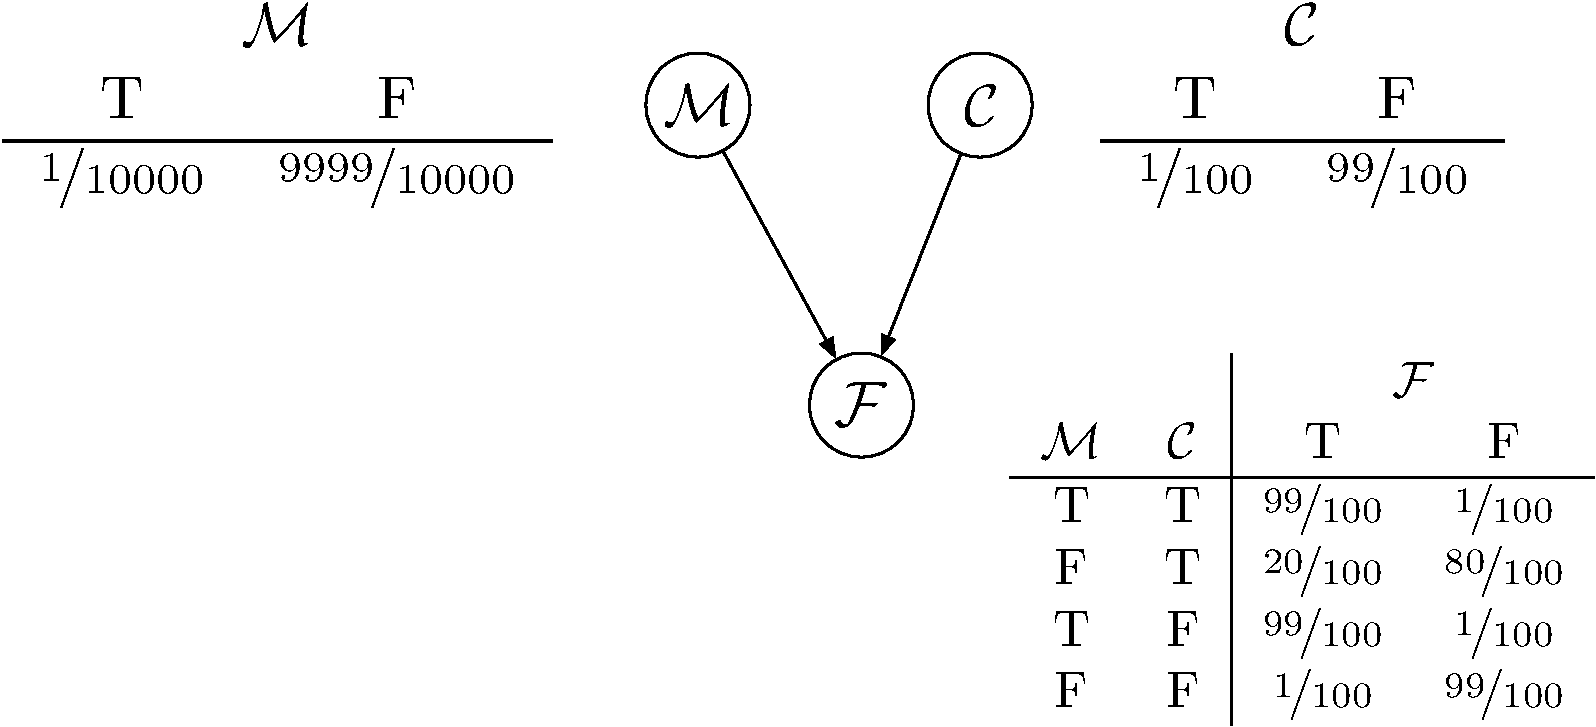
\includegraphics[width=0.6\linewidth]{figures/medicaldiagnosis}
\end{center}
\bes
\item Determine $p(\mathcal{C}|\mathcal{F})$
\begin{boxedsolution}
You can also do this by applying Bayes' Rule first as we did in assignment 2.
\begin{align}
p(\mathcal{C}|\mathcal{F}) &= \frac{p(\mathcal{C}, \mathcal{F})}{p(\mathcal{F})} & \mbox{law of conditional probability} \nonumber \\
p(\mathcal{F}) &= p(\mathcal{F}, \mathcal{C}, \mathcal{M}) + p(\mathcal{F}, \mathcal{C}, \neg \mathcal{M}) + p(\mathcal{F}, \neg \mathcal{C}, \mathcal{M}) + p(\mathcal{F}, \neg \mathcal{C}, \neg \mathcal{M}) &\mbox{marginalize over $\mathcal{M}$ and $\mathcal{C}$}\nonumber \\
&= p(\mathcal{C})p(\mathcal{M})p(\mathcal{F}|\mathcal{M},\mathcal{C}) + p(\mathcal{C})p(\neg \mathcal{M})p(\mathcal{F}|\neg \mathcal{M},\mathcal{C}) \nonumber \\
&\hspace{0.5in}+p(\neg \mathcal{C})p(\mathcal{M})p(\mathcal{F}|\mathcal{M},\neg \mathcal{C}) +p(\neg \mathcal{C})p(\neg \mathcal{M})p(\mathcal{F}|\neg \mathcal{M},\neg \mathcal{C}) & \mbox{factorize: children given parents} \nonumber \\
&= 0.012 \nonumber \\
p(\mathcal{C}, \mathcal{F}) &= p(\mathcal{C}, \mathcal{F}, \mathcal{M})  + p(\mathcal{C}, \mathcal{F}, \neg \mathcal{M}) &\mbox{marginalize over $\mathcal{M}$} \nonumber \\
&= p(\mathcal{C})p(\mathcal{M}) p(\mathcal{F}|\mathcal{M}, \mathcal{C}) + p(\mathcal{C})p(\neg \mathcal{M}) p(\mathcal{F}| \neg \mathcal{M}, \mathcal{C})& \mbox{factorize: children given parents} \nonumber \\
&= 0.002 \nonumber \\
p(\mathcal{C}|\mathcal{F}) &=  0.1667 &\mbox{use the first equation in this box} \nonumber
\end{align}
\end{boxedsolution}
\item Determine $p(\mathcal{C}|\mathcal{F}, \mathcal{M})$.  Why is the effect that conditioning on $\mathcal{M}$ known as \emph{explaining away}?
\begin{boxedsolution}
You can also do this by applying Bayes' Rule first as we did in assignment 2.
\begin{align}
p(\mathcal{C}|\mathcal{F}, \mathcal{M}) &= \frac{p(\mathcal{C}, \mathcal{F}, \mathcal{M})}{p(\mathcal{F}, \mathcal{M})}& \mbox{law of conditional probability} \nonumber \\
p(\mathcal{F}, \mathcal{M}) &= p(\mathcal{C}, \mathcal{F}, \mathcal{M}) + p(\neg \mathcal{C}, \mathcal{F}, \mathcal{M})&\mbox{marginalize over $\mathcal{C}$} \nonumber \\
&= p(\mathcal{C}) p(\mathcal{M}) p(\mathcal{F}|\mathcal{C}, \mathcal{M}) + p(\neg \mathcal{C}) p(\mathcal{M}) p(\mathcal{F}|\neg\mathcal{C}, \mathcal{M}) & \mbox{factorize: children given parents}\nonumber \\
&= 9.9 \times 10^{-5} \nonumber \\
 p(\mathcal{C}, \mathcal{F}, \mathcal{M}) &= p(\mathcal{C}) p(\mathcal{M}) p(\mathcal{F}|\mathcal{C}, \mathcal{M})  & \mbox{factorize: children given parents}\nonumber \\
 &= 9.9 \times 10^{-7} \nonumber \\
 p(\mathcal{C}|\mathcal{F}, \mathcal{M}) &= \frac{1}{100} &\mbox{use the first equation in this box} \nonumber
\end{align}
The fact that the probability of the patient having a cold dropped by a factor of 16 when we found out they had meningitis is the phenomenon of explaining away.  We call this phenomenon explaining away since knowing that the patient had meningitis explains away the evidence of a fever, rendering it less likely to be caused by a cold.

\end{boxedsolution}
\ees

\noindent If you're interested in exploring this idea further (e.g., in the final project), you can visit a symptom checker (like the \href{https://www.mayoclinic.org/symptom-checker/select-symptom/itt-20009075}{Mayo Clinic symptom checker} or the \href{https://symptoms.webmd.com/default.htm\#/info}{WebMD Symptom Checker}).  Also, consider reading (well probably skimming, it's pretty dense) \href{https://www.ncbi.nlm.nih.gov/pmc/articles/PMC4389712/}{Screening tests: a review with examples}.

\end{exercise}

\section{Fairness Criteria for ML}

\href{https://fairmlbook.org/classification.html}{Chapter 2} from \emph{Fairness and machine learning} laid out some formal frameworks for fairness.  In all of these definitions, we refer to the following random variables.

\vspace{1em}
\begin{tabular}{c | c}
\textbf{Variable} & \textbf{Meaning} \\
\hline
$R$ & This is the prediction, or response, of the algorithm (e.g., predict recidivate) \\
$Y$ & This is the actual outcome (e.g., did the person recidivate or not) \\
$A$ & This is a sensitive attribute (e.g., it might encode the race of the person being evaluated)
\end{tabular}


\bi
\item Independence: $R \condindep A$.  This requires that the prediction is independent of the sensitive attribute (without conditioning on anything).  Suppose $R$ is binary (e.g., $R=1$ if you approve someone for a loan and $R=0$ otherwise).  Further, suppose $A$ can take on two values $A=a$ corresponds to some group of people and $A=b$ corresponds to another group of people.
\begin{align}
p(R=1\mid A=a) = P(R=1 \mid A=b)
\end{align}
This means that the loan approval rate must be identical for both groups (irrespective of any correlations between being a member of these groups and other variables that may be relevant for predicting the riskiness of a loan).

\item Separation: $R \condindep A \mid Y$.  This condition requires that the response and the sensitive attribute must be independent given the actual outcome.  Supposing that $R$ is binary (e.g., loan approved or not), $A$ can take on two values ($a$ or $b$), and $Y$ is binary (e.g., $Y=1$ means loan was repaid, $Y=0$ means loan was defaulted upon), we require the following must hold.

\begin{align}
p(R=1 \mid A=a, Y=1) &= p(R=1 \mid A=b, Y=1) \label{eq:tpr} \\
p(R=1 \mid A=a, Y=0) &= p(R=1 \mid A=b, Y=0) \label{eq:fpr} \\
p(R=0 \mid A=a, Y=1) &= p(R=0 \mid A=b, Y=1) \label{eq:fnr} \\
p(R=0 \mid A=a, Y=0) &= p(R=0 \mid A=b, Y=0) \label{eq:tnr}
\end{align}
These equations state that the true positive rate (Equation~\ref{eq:tpr}), false positive rate (Equation~\ref{eq:fpr}), false negative rate (Equation~\ref{eq:fnr}), and true negative rate (Equation~\ref{eq:tnr}) must be equal for group $A=a$ and group $A=b$.  This was the definition of fairness that Propublica used in their analysis.

\item Sufficiency: $Y \condindep A\mid R$.  This condition requires that the outcome and the attribute must be conditionally independent given the algorithm's prediction.   Supposing that $R$ is binary (e.g., loan approved or not), $A$ can take on two values ($a$ or $b$), and $Y$ is binary (e.g., $Y=1$ means loan was repaid, $Y=0$ means loan was defaulted upon), we require the following must hold.

\begin{align}
p(Y=1 \mid A=a, R=1) &= p(Y=1 \mid A=b, R=1) \label{eq:ppv} \\
p(Y=0 \mid A=a, R=0) &= p(Y=0 \mid A=b, R=0) \label{eq:npv}
\end{align}
These equations state that the positive predictive value (Equation~\ref{eq:ppv}) and negative predictive value (Equation~\ref{eq:npv}) must be equal for group $A=a$ and group $A=b$.  This was the definition of fairness that NorthPointe used in their analysis
\ei

\section{Na\"ive Bayes}

The Na\"ive Bayes model can be described using the following BN.

\begin{center}
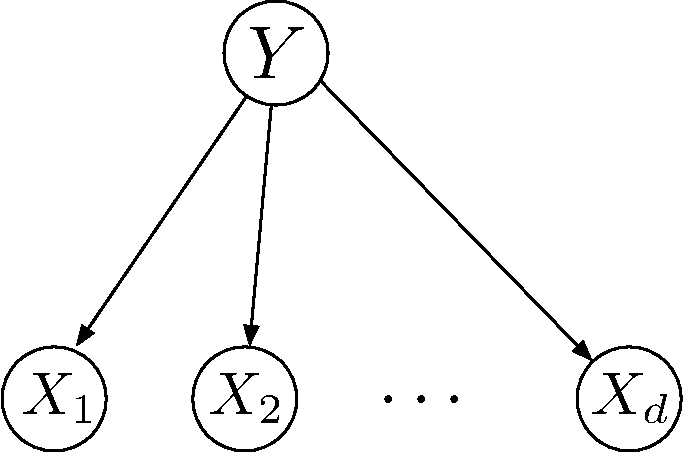
\includegraphics[width=0.3\linewidth]{../02/figures/naivebayesgm}
\end{center}

Remember, that in order to define the BN we need to also specify the conditional probability tables (the probability of each node conditioned on its parents).  For the Na\"ive Bayes model this consists of the following probabilities.

\bi
\item If $Y$ is a random variable, we need $p(Y=i)$ (for all possible values, $i$, that $Y$ could take on).  If $\mathcal{Y}$ is an event, we would need $p(\mathcal{Y})$.
\item If the $X_i$'s are random variables, we need $p(X_i=j | Y=k)$ (for all values, $k$, that $Y$ can take on and all possible values, $j$, that the $X_i$ can take on).  If $\mathcal{X}_i$ is an event, we would need $p(\mathcal{X}_i \mid \mathcal{Y})$ and $p(\mathcal{X}_i \mid \neg \mathcal{Y})$.
\ei

As a motivating example, let's look back at the Titanic dataset from the last module.  A potential BN for the Titanic dataset is shown below.

\begin{center}
\includegraphics[width=0.8\linewidth]{../02/figures/titanicbn}
\end{center}

You'll notice that one of the nodes in this graph is a random variable (\emph{fare class}) and the rest are events (\emph{survived}, \emph{male}, and \emph{young}).  The conditional probabilities were determined using the technique of maximum likelihood estimation (MLE) (which we will describe later).  In this case, MLE simply consists of counting the number of times one of the nodes takes on a particular value when the parent also takes a particular value and normalizing over all possible values the node can take on (more on this in the next section).

\section{Maximum Likelihood Estimation}

In assignment 4, we derived the maximum likelihood estimates for the parameters of the Na\"ive Bayes model.  Rather than redo the derivation here, we're going to do two things.  First, we're going to derive maximum likelihood estimates for a simpler problem.  Next, we're going to apply the maximum likelihood technique to data from the Titanic network.  We hope that these two things will help you wrap your minds around MLE.

\subsection{Flipping Coins}

Suppose we have a coin and we want to know what the probability of it coming up heads is.  Let's call the probability that the coin comes up heads $\Theta$.  Suppose we flip the coin $n$ times.  Let's define a random variable $X_i$ that takes on value $1$ when the coin comes up heads and value $0$ when the coin comes up tails.  We'll use lower case $x_i$ to reference the specific value that we observed for the $i$th flip.  We'd like to determine the maximum likelihood estimate of $\Theta$.  We can write this goal formally using the following equation.


\begin{align}
\Theta^\star &= \argmax_{\Theta} p(X_1 = x_1, X_2 = x_2, \ldots, X_n = x_n | \Theta)
\end{align} 

We can simplify the equation above by making the \href{https://en.wikipedia.org/wiki/Independent_and_identically_distributed_random_variables}{independently and identically distributed (i.i.d.) assumption}.  That is, we'll assume that once we know our model parameter, $\Theta$, each of the random variables $X_i$ is conditionally independent of any other random variable $X_j$.  More formally, we have $X_i \condindep X_j~|~\Theta$ for all $i \neq j$.  Intuitively this means that once we know the bias of the coin, the outcome of each flip has no bearing on the outcome of any other flips.  Applying the i.i.d. assumption gives us

\begin{align}
\Theta^\star &= \argmax_{\Theta} p(X_1 = x_1 | \Theta) p(X_2 = x_2 | \Theta) \ldots p(X_n = x_n | \Theta) \enspace .
\end{align}

We can now take the log of the expression inside of our $\argmax$ without affecting the maximum value.


\begin{align}
\Theta^\star &= \argmax_{\Theta} \log \left ( p(X_1 = x_1 | \Theta) p(X_2 = x_2 | \Theta) \ldots p(X_n = x_n | \Theta) \right) \nonumber \\
&= \argmax_{\Theta} \sum_{i=1}^n \log  p(X_i = x_i | \Theta)
\end{align}

The term $p(X_i = x_i | \Theta)$ will either be $\Theta$ if $x_i$ is 1 or $1-\Theta$ if $x_i$ is 0.  We can indicate this in our equation by using the indicator function, $\mathbb{I}$, that takes on value 1 when the condition inside is true and 0 when the condition inside is false.

\begin{align}
\Theta^\star &= \argmax_{\Theta} \sum_{i=1}^n \left ( \mathbb{I} [ x_i =1] \log \Theta  + \mathbb{I}[x_i = 0]  \log\left (1-  \Theta \right) \right) \label{eq:mlecoin}
\end{align}

Examining Equation~\ref{eq:mlecoin}, we can see that the value inside the summation only depends on whether $x_i$ is 1 or 0.  Therefore, if $n_{H}$ is the number of heads we observed (heads corresponds to $x_i = 1$) and $n_{T}$ is the number of tails we observed (tails corresponds to $x_i = 0$), we can rewrite Equation~\ref{eq:mlecoin} as


\begin{align}
\Theta^\star &= \argmax_{\Theta} n_H \log \Theta  + n_T  \log\left (1-  \Theta \right) \label{eq:mlecoincount} \enspace .
\end{align}

We can solve this equation by taking the derivative with respect to $\Theta$ and setting it to 0 (in Exercise 1 on Assignment 4 we had to use Lagrange multipliers since it was a harder problem; we don't need to do that here).

\begin{align}
\frac{d}{d\Theta} \left ( n_H \log \Theta  + n_T  \log\left (1-  \Theta \right) \right) &=  \frac{n_H}{\Theta} - \frac{n_T}{1-\Theta} \nonumber \\
0 &= \frac{n_H}{\Theta^\star} - \frac{n_T}{1-\Theta^\star} \nonumber & \mbox{$\Theta^\star$ occurs at a critical point, i.e., the derivative is $0$}\\
0 &=  n_H(1-\Theta^\star) - n_T \Theta^\star &\mbox{assuming $\Theta^\star$ is not 0 or 1, we can multiply by $\Theta^\star(1-\Theta^\star)$} \nonumber \\
0&= n_H - n_H \Theta^\star -  n_T \Theta^\star \nonumber \\
(n_H + n_T) \Theta^\star &= n_H \nonumber \\
\Theta^\star &= \frac{n_H}{n_H + n_T} \nonumber \\
\end{align}

While there's a lot of math to get to this final answer (which, tells us to estimate $\Theta^\star$ as the fraction of heads observed in the training data... pretty reasonable!) the steps are very formulaic.
\be
\item Write down the likelihood of the data given the parameters.
\item Simplify the likelihood and substitute in the parameters (the parameters will be symbolic at this point, e.g., $\Theta$).
\item Solve for the optimal value of the parameters (e.g., using Lagrange multipliers or setting derivative to 0 to find a critical point).
\ee

\subsection{MLE and the Titanic}

Some of you requested an example of applying the equations that we worked out in Assignment 4 to an actual example of Na\"ive Bayes.  In that spirit, we will use training data to fit the parameters of our Titanic BN.


The MLE equations that we derived in Assignment 4 are as follows.

\bi
\item To fit the parameters for the outcome variables $Y$, we can use this equation.
\begin{align}
p(Y=i |  \mathbf{\Theta^\star}) = \Theta^\star(i) &= \frac{\mbox{ycount}(i)}{\sum_{j=1}^c \mbox{ycount}(j)}
\end{align}
\item  To fit the conditional probabilities of the features (e.g., young, male, and fare class), we can use the following equation.
\begin{align}
p(X_j = k \mid Y=i , \mathbf{\Theta^\star}) = \Theta_j^\star(k|i) &= \frac{\mbox{xcount}_j(k|i)}{\sum_{u=1}^r \mbox{xcount}_j(u|i)}
\end{align}
\ei

Let's apply these equations to the Titanic BN (the BN is shown earlier in this document).

\bi
\item To determine $p(\mathcal{S})$ we need to count up the number of times each possible outcome occurred.  We can use $\mbox{ycount}(\mathcal{S})$ and  $\mbox{ycount}(\neg \mathcal{S})$ to denote the number of passengers who survived versus didn't survive.
\begin{align}
p(\mathcal{S}) &= \frac{\mbox{ycount}(\mathcal{S})}{\mbox{ycount}(\mathcal{S}) + \mbox{ycount}(\neg \mathcal{S})} \nonumber \\
&= \frac{342}{342+549} \nonumber \\
&= \frac{342}{891} \nonumber
\end{align}
$p(\neg \mathcal{S})$ could be determined similarly, or you could just use $1-p(\mathcal{S})$.

\item In order to determine $p(\mathcal{M} | \mathcal{S})$ and $p(\mathcal{M}|\neg \mathcal{S})$, we need to know four counts: $\mbox{xcount}(\mathcal{M}| \mathcal{S}), \mbox{xcount}(\neg \mathcal{M}| \mathcal{S}), \mbox{xcount}(\mathcal{M}|\neg \mathcal{S})$, and $\mbox{xcount}(\neg \mathcal{M}|\neg \mathcal{S})$ (note: we dropped the subscripts on $\mbox{xcount}$ since it is clear from the arguments which node in the BN we're talking about).

\begin{align}
\Theta^\star(\mathcal{M}|  \mathcal{S}) &= \frac{\mbox{xcount}(\mathcal{M}| \mathcal{S})}{\mbox{xcount}(\mathcal{M}| \mathcal{S}) + \mbox{xcount}(\neg \mathcal{M}|  \mathcal{S}) } \nonumber \\
&= \frac{109}{109+233} \nonumber \\
&= \frac{109}{342} \nonumber
\end{align}

\begin{align}
\Theta^\star(\mathcal{M}| \neg \mathcal{S}) &= \frac{\mbox{xcount}(\mathcal{M}| \neg \mathcal{S})}{\mbox{xcount}(\mathcal{M}| \neg \mathcal{S}) + \mbox{xcount}(\neg \mathcal{M}| \neg \mathcal{S}) } \nonumber \\
&= \frac{468}{468+81} \nonumber \\
&= \frac{468}{549} \nonumber
\end{align}

\begin{exercise}
Apply the formulas to determine the probabilities of $\mathcal{Y}$ and $C$ given $\mathcal{S}$.  Here are the relevant counts.

\bi
\item $\mbox{xcount}(\mathcal{Y}|  \mathcal{S}) = 27$,  $\mbox{xcount}(\neg \mathcal{Y}|  \mathcal{S}) = 315$
\item $\mbox{xcount}(\mathcal{Y}| \neg \mathcal{S}) = 13$,  $\mbox{xcount}(\neg \mathcal{Y}| \neg \mathcal{S}) = 536$
\item $\mbox{xcount}(C=1 | \mathcal{S}) = 136$, $\mbox{xcount}(C=2 | \mathcal{S}) = 87$, $\mbox{xcount}(C=3 | \mathcal{S}) = 119$
\item $\mbox{xcount}(C=1 | \neg \mathcal{S}) = 80$, $\mbox{xcount}(C=2 | \neg \mathcal{S}) = 97$, $\mbox{xcount}(C=3 | \neg \mathcal{S}) = 372$
\ei
\begin{boxedsolution}
We can apply the same steps for $\mathcal{Y}$ as we did for $\mathcal{M}$.
\begin{align}
\Theta^\star(\mathcal{Y}| \mathcal{S}) &= \frac{\mbox{xcount}(\mathcal{Y}| \mathcal{S})}{\mbox{xcount}(\mathcal{Y}| \mathcal{S}) + \mbox{xcount}(\neg \mathcal{Y}|  \mathcal{S}) } \nonumber \\
&= \frac{27}{27+315} \nonumber \\
&= \frac{27}{342} \nonumber \\
\Theta^\star(\mathcal{Y}| \neg \mathcal{S}) &= \frac{\mbox{xcount}(\mathcal{Y}| \neg \mathcal{S})}{\mbox{xcount}(\mathcal{Y}| \neg\mathcal{S}) + \mbox{xcount}(\neg \mathcal{Y}| \neg \mathcal{S}) } \nonumber \\
&= \frac{13}{13+536} \nonumber \\
&= \frac{13}{549}
\end{align}
Due to weird formatting when we didn't do this, the solution will be continued in a second green box.
\end{boxedsolution}

\begin{boxedsolution}
Computing the parameters for $C$ is a little bit harder since we have to consider the 3 different values that C could take on.

\begin{align}
\Theta^\star(C=1 | \mathcal{S}) &= \frac{\mbox{xcount}(C=1| \mathcal{S})}{\mbox{xcount}(C=1| \mathcal{S}) + \mbox{xcount}(C=2| \mathcal{S})  + \mbox{xcount}(C=3 | \mathcal{S}) } \nonumber \\
&= \frac{136}{136+87+119} \nonumber \\
&= \frac{136}{342} \nonumber \\
\Theta^\star(C=2 | \mathcal{S}) &= \frac{\mbox{xcount}(C=2| \mathcal{S})}{\mbox{xcount}(C=1| \mathcal{S}) + \mbox{xcount}(C=2| \mathcal{S})  + \mbox{xcount}(C=3|  \mathcal{S}) } \nonumber \\
&= \frac{87}{136+87+119} \nonumber \\
&= \frac{87}{342} \nonumber \\
\Theta^\star(C=3 | \mathcal{S}) &= \frac{\mbox{xcount}(C=3| \mathcal{S})}{\mbox{xcount}(C=1| \mathcal{S}) + \mbox{xcount}(C=2| \mathcal{S})  + \mbox{xcount}(C=3 | \mathcal{S}) } \nonumber \\
&= \frac{119}{136+87+119} \nonumber \\
&= \frac{119}{342} \nonumber \\
\Theta^\star(C=1 | \neg \mathcal{S}) &= \frac{\mbox{xcount}(C=1| \neg\mathcal{S})}{\mbox{xcount}(C=1|\neg \mathcal{S}) + \mbox{xcount}(C=2| \neg\mathcal{S})  + \mbox{xcount}(C=3|\neg  \mathcal{S}) } \nonumber \\
&= \frac{80}{80 + 97 + 372} \nonumber \\
&= \frac{80}{549} \nonumber \\
\Theta^\star(C=2 | \neg \mathcal{S}) &= \frac{\mbox{xcount}(C=2| \neg\mathcal{S})}{\mbox{xcount}(C=1| \neg\mathcal{S}) + \mbox{xcount}(C=2| \neg\mathcal{S})  + \mbox{xcount}(C=3 |\neg \mathcal{S}) } \nonumber \\
&= \frac{97}{80 + 97 + 372} \nonumber \\
&= \frac{97}{549} \nonumber \\
\Theta^\star(C=3 | \neg \mathcal{S}) &= \frac{\mbox{xcount}(C=3| \neg\mathcal{S})}{\mbox{xcount}(C=1| \neg\mathcal{S}) + \mbox{xcount}(C=2| \neg\mathcal{S})  + \mbox{xcount}(C=3 | \neg\mathcal{S}) } \nonumber \\
&= \frac{372}{80 + 97 + 372} \nonumber \\
&= \frac{372}{549} \nonumber 
\end{align}

\end{boxedsolution}

\end{exercise}

\ei



\section{N-Grams}
This was primarily coding based, so we don't have too much here.  Here are some basic ideas to remember about n-grams.

\bi
\item N-Grams consist of N continuous symbols from a sequence.  A common example of a sequence is text where the symbols are words.  $N=2$ gives us, as a special case, the bigram model and $N=1$ gives us, as a special case, the unigram model.
\item N-Grams can be used as features to represent a sequence (e.g., encoding the presence or absence of a particular N-Gram to summarize a document).
\item These features can be used to classify the document or to compute various conditional probabilities (e.g., the probability that some symbol follows another).
\ei

\section{Are we missing anything?}
Keep in mind that this document's scope is within the math / algorithms part of this class (not on the context and ethics or programming side).  Comment on NB here to request stuff to add. 

\end{document}
